%==============================================================
%  EE201 -- Circuit Theory I
%  Lecture 6 : Dependent Sources and the Ideal Transformer
%  M. Mert Ankaralı, METU EEE
%
%  Compile:  ./build.sh      (or: pdflatex EE201_Lecture_6.tex, twice)
%==============================================================
\documentclass[11pt,a4paper]{article}

%-------------------- packages --------------------------------
\usepackage[T1]{fontenc}
\usepackage[utf8]{inputenc}
\usepackage[english]{babel}
\usepackage{lmodern}
\usepackage[margin=2.3cm,top=2.0cm,bottom=1.9cm,headheight=14pt,headsep=9pt]{geometry}
\usepackage{amsmath,amssymb}
\usepackage{array,booktabs,tabularx}
\usepackage{enumitem}
\usepackage[table]{xcolor}
\usepackage{fancyhdr}
\usepackage{titlesec}
\usepackage{graphicx}
\usepackage[most]{tcolorbox}
\usepackage{tikz}
\usepackage[american,siunitx]{circuitikz}
\usetikzlibrary{arrows.meta,positioning,calc,decorations.pathmorphing,decorations.pathreplacing,decorations.markings,patterns,shapes.geometric}
\usepackage[colorlinks=true,allcolors=metured,breaklinks=true]{hyperref}

%-------------------- colour system ---------------------------
% One colour per physical quantity, used identically in the slides.
\definecolor{metured}{RGB}{155,27,48}    % headings, structure
\definecolor{metugray}{RGB}{88,89,91}
\definecolor{ccur}{RGB}{0,102,170}       % CURRENT  -- blue
\definecolor{cvolt}{RGB}{214,120,0}      % VOLTAGE  -- orange
\definecolor{cpow}{RGB}{23,128,74}       % POWER / ENERGY -- green
\definecolor{ccharge}{RGB}{124,60,160}   % CHARGE   -- purple
\definecolor{cflux}{RGB}{0,138,138}      % FLUX -- teal
\definecolor{boxgray}{RGB}{245,245,245}
\definecolor{copper}{RGB}{184,98,30}

\newcommand{\Icol}[1]{\textcolor{ccur}{#1}}
\newcommand{\Vcol}[1]{\textcolor{cvolt}{#1}}
\newcommand{\Pcol}[1]{\textcolor{cpow}{#1}}
\newcommand{\Qcol}[1]{\textcolor{ccharge}{#1}}
\newcommand{\Fcol}[1]{\textcolor{cflux}{#1}}

%-------------------- units (no siunitx dependency) -----------
\newcommand{\uni}[1]{\,\mathrm{#1}}
\newcommand{\A}{\uni{A}}   \newcommand{\V}{\uni{V}}
\newcommand{\W}{\uni{W}}   \newcommand{\J}{\uni{J}}
\newcommand{\Cb}{\uni{C}}  \newcommand{\s}{\uni{s}}
\newcommand{\Sie}{\uni{S}} \newcommand{\Wb}{\uni{Wb}}

%-------------------- layout ----------------------------------
\pagestyle{fancy}
\fancyhf{}
\lhead{\small\textcolor{metugray}{EE201 -- Circuit Theory I}}
\rhead{\small\textcolor{metugray}{Lecture 6: Dependent Sources and the Ideal Transformer}}
\cfoot{\small\thepage}
\renewcommand{\headrulewidth}{0.4pt}

\titleformat{\section}{\large\bfseries\color{metured}}{\thesection.}{0.6em}{}
\titleformat{\subsection}{\normalsize\bfseries\color{metugray}}{\thesubsection.}{0.6em}{}
\titlespacing*{\section}{0pt}{1.4ex plus .3ex}{0.7ex}
\titlespacing*{\subsection}{0pt}{1.1ex plus .2ex}{0.5ex}

\setlist[itemize]{itemsep=2pt,topsep=3pt,parsep=0pt,leftmargin=1.5em}
\setlist[enumerate]{itemsep=2pt,topsep=3pt,parsep=0pt,leftmargin=1.7em}
\setlength{\parindent}{0pt}
\setlength{\parskip}{0.7ex plus .1ex}
\raggedbottom
\widowpenalty=10000
\clubpenalty=10000
\brokenpenalty=10000

%-------------------- boxes -----------------------------------
\newtcolorbox{definitionbox}[1]{enhanced,
  colback=metured!4, colframe=metured, boxrule=0.9pt,
  fonttitle=\bfseries, title={#1}, arc=2pt,
  left=7pt,right=7pt,top=5pt,bottom=5pt, before skip=7pt, after skip=7pt,
  before upper={\setlength{\parskip}{0.6ex plus .1ex}}}

\newtcolorbox{ideabox}[1][Key idea]{enhanced,
  colback=ccur!5, colframe=ccur, boxrule=0.9pt,
  fonttitle=\bfseries, title={#1}, arc=2pt,
  left=7pt,right=7pt,top=5pt,bottom=5pt, before skip=7pt, after skip=7pt,
  before upper={\setlength{\parskip}{0.6ex plus .1ex}}}

\newtcolorbox{examplebox}[1][Example]{enhanced,
  colback=cpow!4, colframe=cpow, boxrule=0.9pt,
  fonttitle=\bfseries, title={#1}, arc=2pt,
  left=7pt,right=7pt,top=5pt,bottom=5pt, before skip=7pt, after skip=7pt,
  before upper={\setlength{\parskip}{0.6ex plus .1ex}}}

\newtcolorbox{cautionbox}[1][Careful]{enhanced,
  colback=cvolt!6, colframe=cvolt, boxrule=0.9pt,
  fonttitle=\bfseries, title={#1}, arc=2pt,
  left=7pt,right=7pt,top=5pt,bottom=5pt, before skip=7pt, after skip=7pt,
  before upper={\setlength{\parskip}{0.6ex plus .1ex}}}

%-------------------- circuitikz defaults ---------------------
\ctikzset{bipoles/length=0.9cm, color=black,
          label/align=straight,
          bipoles/vsourceam/height=0.85, bipoles/vsourceam/width=0.85}
\tikzset{
  curarr/.style={-{Stealth[length=2.6mm]}, ccur, very thick},
  flowarr/.style={-{Stealth[length=3mm]}, metured, very thick},
  pol/.style={font=\small, text=cvolt},
  iar/.style={-{Stealth[length=2.4mm]}, ccur, very thick},
  glab/.style={font=\footnotesize, text=metured},
  ttl/.style={font=\scriptsize\bfseries, text=metugray},
  capn/.style={font=\scriptsize, text=metugray, align=center},
  surf/.style={draw=cpow, very thick, dashed, rounded corners=6pt},
  ampbox/.style={draw=metured!70, thick, dashed, rounded corners=5pt},
  dotm/.style={circle, fill=black, inner sep=0pt, minimum size=4.2pt},
  core/.style={line width=1.1pt, metugray},
}
\newcommand{\ohm}{\,\Omega}
\newcommand{\kohm}{\,\mathrm{k}\Omega}

%  A two-winding ideal-transformer symbol between (#1,0)--(#1,#2) on the left and
%  (#1+1.6,0)--(#1+1.6,#2) on the right; dots at the top of both windings.
\newcommand{\xfmr}[2]{%
  \begin{scope}[xshift=#1 cm]
    \ctikzset{bipoles/length=1.35cm}
    \draw (0,0) to[L] (0,#2);
    \draw (1.6,#2) to[L] (1.6,0);
    \draw[core] (0.72,-0.05) -- (0.72,#2+0.05);
    \draw[core] (0.88,-0.05) -- (0.88,#2+0.05);
    \node[dotm] at (0.36,#2-0.2) {};
    \node[dotm] at (1.24,#2-0.2) {};
  \end{scope}}

%==============================================================
\begin{document}

%-------------------- title block -----------------------------
\begin{center}
\begin{tcolorbox}[enhanced, colback=metured!5, colframe=metured, boxrule=1pt,
                  arc=3pt, left=10pt,right=10pt,top=7pt,bottom=7pt, width=\textwidth]
\begin{center}
  {\small\scshape Middle East Technical University}\\[2pt]
  {\small\scshape Department of Electrical and Electronics Engineering}\\[7pt]
  {\Large\bfseries\color{metured} EE201 -- Circuit Theory I}\\[4pt]
  {\large\bfseries Lecture 6: Dependent Sources and the Ideal Transformer}\\[6pt]
  {\small M. Mert Ankaralı}
\end{center}
\end{tcolorbox}
\end{center}
\vspace{-0.5em}

\begin{center}
\small
\begin{tabular}{@{}l l@{}}
\toprule
\multicolumn{2}{@{}l}{\textbf{Colour code used in these notes and in the slides}}\\
\midrule
\Icol{$\blacksquare$}~current $i$ \quad \Vcol{$\blacksquare$}~voltage $v$ &
\Pcol{$\blacksquare$}~power $p$ \quad \Fcol{$\blacksquare$}~magnetic flux $\Phi$\\
\bottomrule
\end{tabular}
\end{center}

%==============================================================
\section{Sources controlled from elsewhere}

The sources of Lecture~3 decide their own value. A $12\V$ source holds $12\V$ whatever the
rest of the circuit does. Today's sources do not: their value is set by a voltage or a
current \emph{somewhere else} in the circuit. They are how an amplifier, a transistor or an
op-amp enters a circuit diagram.

\begin{definitionbox}{Dependent (controlled) source}
A \textbf{dependent source} is a voltage or current source whose value is a function of a
voltage or current in \emph{another} branch of the circuit, the \textbf{controlling
variable}. When the function is a constant times the controlling variable, it is a
\textbf{linear} dependent source. All dependent sources in EE201 are linear.
\end{definitionbox}

The symbol is a \textbf{diamond}. A circle means the source decides its own value; a
diamond means it copies, scaled, a variable from elsewhere.

\begin{center}
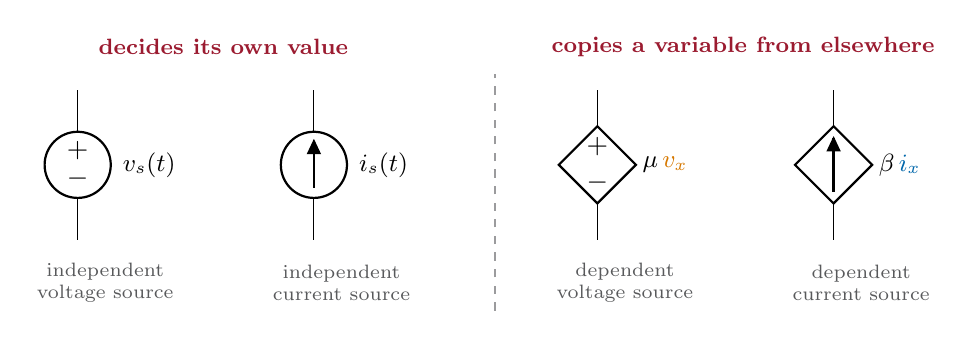
\begin{tikzpicture}[scale=1.0]
  \begin{scope}
    \draw (0,0) to[american voltage source, invert] (0,1.9);
    \node[font=\small, right] at (0.45,0.95) {$v_s(t)$};
    \node[capn] at (0.35,-0.55) {independent\\ voltage source};
  \end{scope}
  \begin{scope}[xshift=3.0cm]
    \draw (0,0) to[american current source] (0,1.9);
    \node[font=\small, right] at (0.45,0.95) {$i_s(t)$};
    \node[capn] at (0.35,-0.55) {independent\\ current source};
  \end{scope}
  \draw[metugray!60, dashed] (5.3,-0.9) -- (5.3,2.1);
  \begin{scope}[xshift=6.6cm]
    \draw (0,0) to[american controlled voltage source, invert] (0,1.9);
    \node[font=\small, right] at (0.45,0.95) {$\mu\,\Vcol{v_x}$};
    \node[capn] at (0.35,-0.55) {dependent\\ voltage source};
  \end{scope}
  \begin{scope}[xshift=9.6cm]
    \draw (0,0) to[american controlled current source] (0,1.9);
    \node[font=\small, right] at (0.45,0.95) {$\beta\,\Icol{i_x}$};
    \node[capn] at (0.35,-0.55) {dependent\\ current source};
  \end{scope}
  \node[font=\footnotesize\bfseries, text=metured] at (1.85,2.45) {decides its own value};
  \node[font=\footnotesize\bfseries, text=metured] at (8.45,2.45) {copies a variable from elsewhere};
\end{tikzpicture}
\end{center}

%==============================================================
\section{The four kinds}

A dependent source senses a voltage or a current, and produces a voltage or a current. That
gives four kinds. The name reads in that order --- what it senses, then what it produces.

\begin{center}
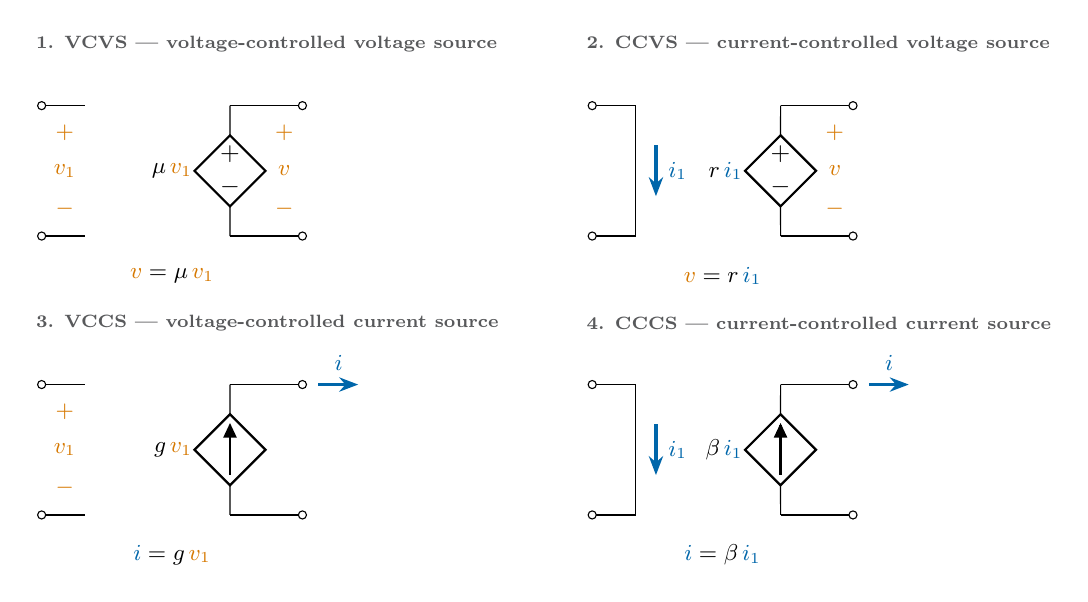
\begin{tikzpicture}[scale=0.92, transform shape]
 % #1 x-shift, #2 y-shift, #3 title, #4 control side (v or i), #5 output (v or i), #6 value, #7 equation
 \foreach \sx/\sy/\ttlx/\ctl/\out/\val/\eqn in {%
   0/0/{1. VCVS --- voltage-controlled voltage source}/v/v/{$\mu\,\Vcol{v_1}$}/{$\Vcol{v} = \mu\,\Vcol{v_1}$},
   7.6/0/{2. CCVS --- current-controlled voltage source}/i/v/{$r\,\Icol{i_1}$}/{$\Vcol{v} = r\,\Icol{i_1}$},
   0/-3.85/{3. VCCS --- voltage-controlled current source}/v/i/{$g\,\Vcol{v_1}$}/{$\Icol{i} = g\,\Vcol{v_1}$},
   7.6/-3.85/{4. CCCS --- current-controlled current source}/i/i/{$\beta\,\Icol{i_1}$}/{$\Icol{i} = \beta\,\Icol{i_1}$}}{
 \begin{scope}[xshift=\sx cm, yshift=\sy cm]
  \node[ttl, anchor=west] at (-0.2,2.65) {\ttlx};
  \if v\ctl
    \draw (0,0) node[ocirc]{} -- (0.6,0); \draw (0,1.8) node[ocirc]{} -- (0.6,1.8);
    \node[pol] at (0.32,1.42) {$+$}; \node[pol] at (0.32,0.38) {$-$};
    \node[pol] at (0.32,0.9) {$v_1$};
  \else
    \draw (0,0) node[ocirc]{} -- (0.6,0) -- (0.6,1.8) -- (0,1.8) node[ocirc]{};
    \draw[iar] (0.88,1.25) -- (0.88,0.55); \node[font=\small, text=ccur] at (1.18,0.9) {$i_1$};
  \fi
  \if v\out
    \draw (2.6,0) to[american controlled voltage source, invert] (2.6,1.8);
    \node[pol] at (3.35,1.42) {$+$}; \node[pol] at (3.35,0.38) {$-$};
    \node[pol] at (3.35,0.9) {$v$};
  \else
    \draw (2.6,0) to[american controlled current source] (2.6,1.8);
    \draw[iar] (3.82,1.8) -- (4.37,1.8); \node[font=\small, text=ccur] at (4.1,2.1) {$i$};
  \fi
  \draw (2.6,1.8) -- (3.6,1.8) node[ocirc]{}; \draw (2.6,0) -- (3.6,0) node[ocirc]{};
  \node[font=\small, left] at (2.2,0.9) {\val};
  \node[font=\small] at (1.8,-0.55) {\eqn};
 \end{scope}}
\end{tikzpicture}
\end{center}

\begin{center}
\small
\begin{tabular}{@{}l l l l@{}}
\toprule
\textbf{Kind} & \textbf{Terminal equation} & \textbf{The constant is called} & \textbf{Unit}\\
\midrule
VCVS & $\Vcol{v} = \mu\,\Vcol{v_1}$ & voltage gain       & none (V/V)\\
CCVS & $\Vcol{v} = r\,\Icol{i_1}$   & transresistance    & ohm, $\Omega$ (V/A)\\
VCCS & $\Icol{i} = g\,\Vcol{v_1}$   & transconductance   & siemens, S (A/V)\\
CCCS & $\Icol{i} = \beta\,\Icol{i_1}$ & current gain     & none (A/A)\\
\bottomrule
\end{tabular}
\end{center}

The unit of the constant is always ``what comes out'' over ``what goes in''. When the two
are different kinds of quantity the name carries \emph{trans-}: a transresistance turns a
current into a voltage, so it is measured in ohms, like a resistance.

\subsection{The sensing side}

In each picture the left-hand pair of terminals is where the source senses its controlling
variable. It senses it without disturbing anything:
\begin{itemize}
  \item to sense a \Vcol{voltage} it is an \textbf{open circuit} --- it draws no current;
  \item to sense a \Icol{current} it is a \textbf{short circuit} --- it takes no voltage.
\end{itemize}
In a real circuit diagram the sensing side is almost never drawn. The controlling
variable is simply the voltage across, or the current through, some element that is
already there, and the diagram labels it: $\Vcol{v_x}$, $\Icol{i_x}$, $\Icol{i_1}$.

%==============================================================
\section{Why we need them}

A dependent source is the simplest model of anything that \emph{amplifies}. The picture
below is how an amplifier usually appears in a circuit diagram.

\begin{center}
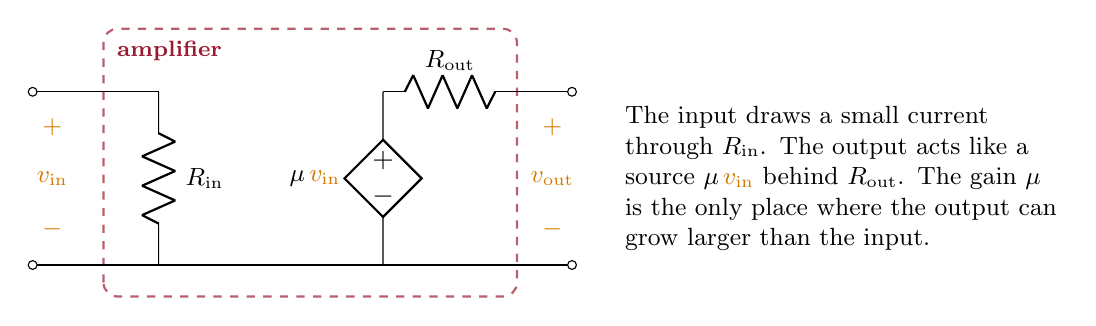
\begin{tikzpicture}[scale=1.0]
  \draw[ampbox] (0.5,-0.4) rectangle (5.75,3.0);
  \node[font=\footnotesize\bfseries, text=metured, anchor=north west] at (0.55,2.97) {amplifier};
  \draw (-0.4,2.2) node[ocirc]{} -- (1.2,2.2);
  \draw (-0.4,0) node[ocirc]{} -- (1.2,0);
  \draw (1.2,0) to[R] (1.2,2.2);
  \node[font=\small, right] at (1.42,1.1) {$R_{\mathrm{in}}$};
  \node[pol] at (-0.15,1.75) {$+$}; \node[pol] at (-0.15,0.45) {$-$};
  \node[pol] at (-0.15,1.1) {$v_{\mathrm{in}}$};
  \draw (4.05,0) to[american controlled voltage source, invert] (4.05,2.2);
  \node[font=\small, left] at (3.63,1.1) {$\mu\,\Vcol{v_{\mathrm{in}}}$};
  \draw (4.05,2.2) to[R] (5.75,2.2) -- (6.45,2.2) node[ocirc]{};
  \node[font=\small] at (4.9,2.6) {$R_{\mathrm{out}}$};
  \draw (1.2,0) -- (6.45,0) node[ocirc]{};
  \node[pol] at (6.2,1.75) {$+$}; \node[pol] at (6.2,0.45) {$-$};
  \node[pol] at (6.2,1.1) {$v_{\mathrm{out}}$};
  \node[font=\small, anchor=west, text width=5.5cm] at (7.0,1.1)
    {The input draws a small current through $R_{\mathrm{in}}$. The output acts like a
     source $\mu\,\Vcol{v_{\mathrm{in}}}$ behind $R_{\mathrm{out}}$. The gain $\mu$ is
     the only place where the output can grow larger than the input.};
\end{tikzpicture}
\end{center}

The same idea models real devices. A transistor is modelled with a VCCS or a CCCS; you will
meet both in the electronics courses. An op-amp is a VCVS with an enormous gain,
$\mu \approx 10^5$; it has a chapter of its own later in this course.

%==============================================================
\section{Reading a diagram with a dependent source}

\begin{examplebox}[Example 6.1 --- what the diamond says]
Which equation does the dependent source contribute in this circuit?

\begin{minipage}[c]{0.56\linewidth}
\centering
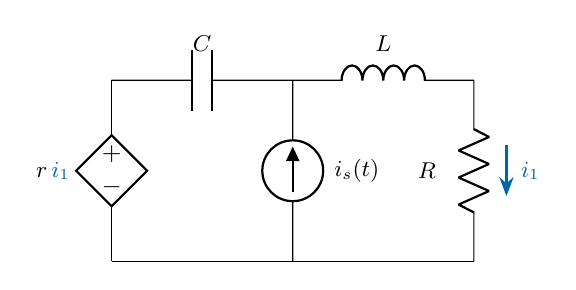
\begin{tikzpicture}[scale=0.92, transform shape]
  \draw (0,0) to[american controlled voltage source, invert] (0,2.5);
  \node[font=\small, left] at (-0.45,1.25) {$r\,\Icol{i_1}$};
  \draw (0,2.5) to[C] (2.5,2.5);
  \node[font=\small] at (1.25,3.0) {$C$};
  \draw (2.5,0) to[american current source] (2.5,2.5);
  \node[font=\small, right] at (2.95,1.25) {$i_s(t)$};
  \draw (2.5,2.5) to[L] (5.0,2.5);
  \node[font=\small] at (3.75,3.0) {$L$};
  \draw (5.0,2.5) to[R] (5.0,0);
  \node[font=\small, left] at (4.6,1.25) {$R$};
  \draw[iar] (5.45,1.6) -- (5.45,0.9); \node[font=\small, text=ccur] at (5.78,1.25) {$i_1$};
  \draw (5.0,0) -- (0,0);
\end{tikzpicture}
\end{minipage}\hfill
\begin{minipage}[c]{0.41\linewidth}
It is a CCVS, so its terminal equation is $\Vcol{v} = r\,\Icol{i_1}$ --- and $\Icol{i_1}$
is the current through $R$. The source sits at the far left; the current it senses flows
at the far right.
\end{minipage}

Count as in Lecture~2: $n = 4$, $b = 5$, so $2b = 10$ unknowns and $b = 5$ terminal
equations. Four of them --- for $C$, $L$, $i_s$ and $R$ --- each speak about one element. The
fifth ties the source's own voltage to another branch's current.
\end{examplebox}

\begin{ideabox}[What is new]
In Lecture~2 every terminal equation described one element \emph{in isolation}. A dependent
source does not: its terminal equation names a variable of another branch. Nothing else
changes. KCL and KVL are the same, and there are still $2b$ equations for $2b$ unknowns.
\end{ideabox}

\begin{cautionbox}[Two meanings of ``controlled'']
In Lecture~3 a resistor was \emph{voltage-controlled} if its current is a function of its
\emph{own} voltage, $\Icol{i} = f(\Vcol{v})$. A voltage-controlled \emph{source} is
different: its value is set by the voltage of \emph{another} branch. The first describes
one element's curve; the second is a link between two branches.
\end{cautionbox}

%==============================================================
\section{Solving circuits with dependent sources}

No new method is needed.

\begin{ideabox}[Recipe]
\begin{enumerate}[leftmargin=1.4em]
  \item Treat the dependent source as if it were independent, with its value written as
        $\mu\Vcol{v_x}$, $r\Icol{i_x}$, $g\Vcol{v_x}$ or $\beta\Icol{i_x}$.
  \item Write KCL, KVL and the terminal equations as usual.
  \item Add one equation that gives the controlling variable in terms of your unknowns.
\end{enumerate}
\end{ideabox}

\begin{examplebox}[Example 6.2 --- an amplifier]
A microphone, $v_s = 50\uni{mV}$ with internal resistance $R_s = 1\kohm$, drives the
amplifier of Section~3 with $R_{\mathrm{in}} = 4\kohm$, $\mu = 100$ and
$R_{\mathrm{out}} = 100\ohm$. The load is $R_L = 400\ohm$. Find $\Vcol{v_L}$, and compare the
power the microphone supplies with the power the load receives.

\begin{center}
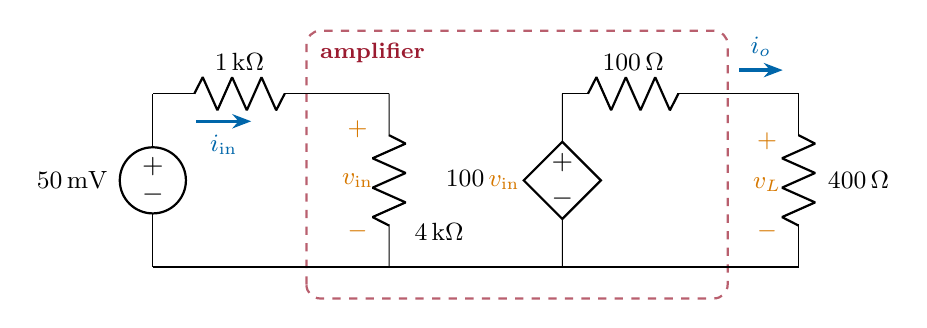
\begin{tikzpicture}[scale=1.0]
  \draw[ampbox] (1.95,-0.4) rectangle (7.3,3.0);
  \node[font=\footnotesize\bfseries, text=metured, anchor=north west] at (2.0,2.97) {amplifier};
  \draw (0,0) to[american voltage source, invert] (0,2.2);
  \node[font=\small, left] at (-0.45,1.1) {$50\uni{mV}$};
  \draw (0,2.2) to[R] (2.2,2.2) -- (3.0,2.2);
  \node[font=\small] at (1.1,2.6) {$1\kohm$};
  \draw[iar] (0.55,1.85) -- (1.25,1.85); \node[font=\small, text=ccur] at (0.9,1.55) {$i_{\mathrm{in}}$};
  \draw (3.0,0) to[R] (3.0,2.2);
  \node[font=\small, anchor=west] at (3.2,0.45) {$4\kohm$};
  \node[pol] at (2.6,1.75) {$+$}; \node[pol] at (2.6,1.1) {$v_{\mathrm{in}}$};
  \node[pol] at (2.6,0.45) {$-$};
  \draw (5.2,0) to[american controlled voltage source, invert] (5.2,2.2);
  \node[font=\small, left] at (4.78,1.1) {$100\,\Vcol{v_{\mathrm{in}}}$};
  \draw (5.2,2.2) to[R] (7.0,2.2) -- (8.2,2.2);
  \node[font=\small] at (6.1,2.6) {$100\ohm$};
  \draw[iar] (7.45,2.5) -- (8.0,2.5); \node[font=\small, text=ccur] at (7.72,2.8) {$i_o$};
  \draw (8.2,2.2) to[R] (8.2,0);
  \node[font=\small, anchor=west] at (8.45,1.1) {$400\ohm$};
  \node[pol] at (7.8,1.6) {$+$}; \node[pol] at (7.8,1.05) {$v_L$}; \node[pol] at (7.8,0.45) {$-$};
  \draw (8.2,0) -- (0,0);
\end{tikzpicture}
\end{center}

\textbf{Input side.} One loop, a divider:
$\Icol{i_{\mathrm{in}}} = 50\uni{mV}/5\kohm = 10\uni{\mu A}$, so
$\Vcol{v_{\mathrm{in}}} = 4\kohm \times 10\uni{\mu A} = 40\uni{mV}$.

\textbf{Output side.} The diamond now has a value: $100 \times 40\uni{mV} = 4\V$. Another
divider: $\Icol{i_o} = 4\V/500\ohm = 8\uni{mA}$, so
\[
  \boxed{\Vcol{v_L} = 400\ohm \times 8\uni{mA} = 3.2\V}, \qquad
  \frac{\Vcol{v_L}}{v_s} = 64 .
\]
The overall gain is $64$, not $100$: part of the signal is lost in $R_s$ and part in
$R_{\mathrm{out}}$.
\end{examplebox}

\begin{examplebox}[Example 6.2, continued --- where the power comes from]
With the PSC on every element:

\begin{center}
\small
\begin{tabular}{@{}l r @{\hspace{2.2em}} l r@{}}
\toprule
\multicolumn{2}{@{}l}{\textbf{input side}} & \multicolumn{2}{l@{}}{\textbf{output side}}\\
\midrule
microphone $v_s$ & $-0.5\uni{\mu W}$ & dependent source & $-32\uni{mW}$\\
$R_s$            & $+0.1\uni{\mu W}$ & $R_{\mathrm{out}}$ & $+6.4\uni{mW}$\\
$R_{\mathrm{in}}$ & $+0.4\uni{\mu W}$ & $R_L$            & $+25.6\uni{mW}$\\
\bottomrule
\end{tabular}
\end{center}

Each side sums to zero. The load receives $25.6\uni{mW}$ while the microphone supplies only
$0.5\uni{\mu W}$ --- $51\,200$ times less. The dependent source supplied the difference. A
real amplifier takes that energy from its power supply, which the model does not draw.

One more detail: the bottom wire is shared, yet it carries no current. Wrap a closed surface
around the input side (Lecture~2): that wire is the only branch crossing it, so its current
is zero. The two sides interact only through $\Vcol{v_{\mathrm{in}}}$.
\end{examplebox}

\begin{examplebox}[Example 6.3 --- when the controlling variable is unknown]
The CCCS pushes $2\Icol{i_x}$ into node $a$, where $\Icol{i_x}$ is the current through the
$2\ohm$ resistor. Find $\Icol{i_x}$ and $\Vcol{v_a}$.

\begin{center}
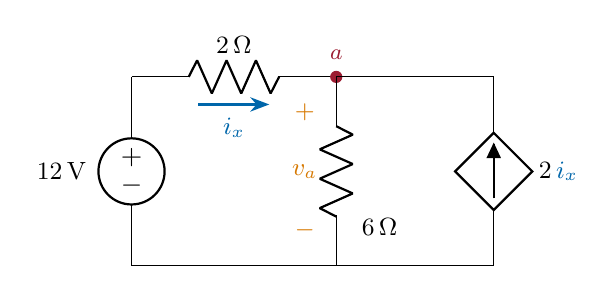
\begin{tikzpicture}[scale=1.0]
  \draw (0,0) to[american voltage source, invert] (0,2.4);
  \node[font=\small, left] at (-0.45,1.2) {$12\V$};
  \draw (0,2.4) to[R] (2.6,2.4);
  \node[font=\small] at (1.3,2.8) {$2\ohm$};
  \draw[iar] (0.85,2.05) -- (1.75,2.05); \node[font=\small, text=ccur] at (1.3,1.75) {$i_x$};
  \fill[metured] (2.6,2.4) circle (2.2pt); \node[glab, above] at (2.6,2.5) {$a$};
  \draw (2.6,0) to[R] (2.6,2.4);
  \node[font=\small, right] at (2.8,0.5) {$6\ohm$};
  \node[pol] at (2.2,1.95) {$+$}; \node[pol] at (2.2,1.2) {$v_a$}; \node[pol] at (2.2,0.45) {$-$};
  \draw (2.6,2.4) -- (4.6,2.4);
  \draw (4.6,0) to[american controlled current source] (4.6,2.4);
  \node[font=\small, right] at (5.05,1.2) {$2\,\Icol{i_x}$};
  \draw (4.6,0) -- (0,0);
\end{tikzpicture}
\end{center}

\textbf{Equations.} Here step 3 is free: $\Icol{i_x}$ is already one of the unknowns.
\[
  \text{KVL:}\quad -12 + 2\Icol{i_x} + \Vcol{v_a} = 0,
  \qquad
  \text{KCL at } a\text{:}\quad -\Icol{i_x} - 2\Icol{i_x} + \frac{\Vcol{v_a}}{6} = 0
  \;\Longrightarrow\; \Vcol{v_a} = 18\,\Icol{i_x} .
\]
\textbf{Solution.} $-12 + 2\Icol{i_x} + 18\Icol{i_x} = 0$, so
\[
  \boxed{\Icol{i_x} = 0.6\A}, \qquad \boxed{\Vcol{v_a} = 10.8\V}.
\]
\textbf{Power check.} The $12\V$ source supplies $7.2\W$. The resistors absorb
$2(0.6)^2 = 0.72\W$ and $10.8^2/6 = 19.44\W$. The CCCS carries $1.2\A$ \emph{out of} its $+$
terminal, so it absorbs $10.8 \times (-1.2) = -12.96\W$:
\[
  -7.2 + 0.72 + 19.44 - 12.96 = 0 .
\]
The $6\ohm$ resistor absorbs more than the independent source supplies. The dependent source
makes up the rest.
\end{examplebox}

\begin{cautionbox}[What a dependent source cannot do]
\textbf{It cannot start anything.} Switch the $12\V$ source of Example~6.3 off. The equations
become $2\Icol{i_x} + \Vcol{v_a} = 0$ and $\Vcol{v_a} = 18\Icol{i_x}$, so
$20\,\Icol{i_x} = 0$: every voltage and current is zero, the dependent source's included.
Without an independent source, all-zero satisfies every equation --- and when the circuit has
a unique solution, that is the solution.\\[3pt]
\textbf{It is never switched off.} Later we will switch sources off one at a time
(superposition, Thévenin equivalents). Only \emph{independent} sources are switched off. A
dependent source stays: its value is not an input, it is part of how the circuit behaves.
\end{cautionbox}

%==============================================================
\section{The ideal transformer}

\subsection{Two coils, one core}

Lecture~1 assumed that no changing magnetic field links the loops of a circuit. Lecture~2
added: when we \emph{want} such a link, we draw it as an element of its own. The transformer
is that element. In Lecture~5 a coil's changing current made a changing field through the
coil itself. Wind two coils on one iron core and the field of each passes through the
other.

\begin{center}
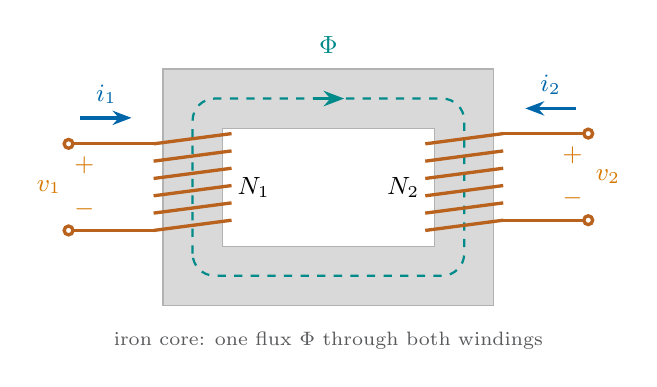
\begin{tikzpicture}[scale=1.0]
  % core
  \fill[gray!30, even odd rule] (0,0) rectangle (4.2,3.0) (0.75,0.75) rectangle (3.45,2.25);
  \draw[gray!60] (0,0) rectangle (4.2,3.0); \draw[gray!60] (0.75,0.75) rectangle (3.45,2.25);
  % flux path
  \draw[cflux, thick, dashed, rounded corners=8pt] (0.375,0.375) rectangle (3.825,2.625);
  \draw[-{Stealth[length=2.6mm]}, cflux, very thick] (1.9,2.625) -- (2.3,2.625);
  \node[font=\small, text=cflux] at (2.1,3.3) {$\Fcol{\Phi}$};
  % windings
  \foreach \y in {0.95,1.17,...,2.05}{
    \draw[copper, very thick] (-0.12,\y) -- (0.87,\y+0.13);
    \draw[copper, very thick] (3.33,\y) -- (4.32,\y+0.13);}
  \draw[copper, very thick] (-0.12,2.05) -- (-1.2,2.05) node[ocirc]{};
  \draw[copper, very thick] (-0.12,0.95) -- (-1.2,0.95) node[ocirc]{};
  \draw[copper, very thick] (4.32,2.18) -- (5.4,2.18) node[ocirc]{};
  \draw[copper, very thick] (4.32,1.08) -- (5.4,1.08) node[ocirc]{};
  \node[font=\small] at (1.15,1.5) {$N_1$};  \node[font=\small] at (3.05,1.5) {$N_2$};
  \node[pol] at (-1.0,1.78) {$+$}; \node[pol] at (-1.0,1.22) {$-$};
  \node[pol] at (-1.45,1.5) {$v_1$};
  \node[pol] at (5.2,1.9) {$+$}; \node[pol] at (5.2,1.36) {$-$};
  \node[pol] at (5.65,1.63) {$v_2$};
  \draw[iar] (-1.05,2.38) -- (-0.4,2.38); \node[font=\small, text=ccur] at (-0.72,2.68) {$i_1$};
  \draw[iar] (5.25,2.5) -- (4.6,2.5); \node[font=\small, text=ccur] at (4.92,2.8) {$i_2$};
  \node[capn] at (2.1,-0.45) {iron core: one flux $\Phi$ through both windings};
\end{tikzpicture}
\end{center}

\subsection{The element}

\begin{definitionbox}{Ideal transformer (two windings)}
With $\Vcol{v_1}$, $\Vcol{v_2}$ positive at the dotted terminals and $\Icol{i_1}$,
$\Icol{i_2}$ entering the dotted terminals,
\[
  \boxed{\;\frac{\Vcol{v_1}}{N_1} = \frac{\Vcol{v_2}}{N_2}\;}
  \qquad\qquad
  \boxed{\;N_1\Icol{i_1} + N_2\Icol{i_2} = 0\;}
\]
$N_1$ and $N_2$ are the numbers of turns. Equivalently,
$\Vcol{v_2} = \dfrac{N_2}{N_1}\,\Vcol{v_1}$ and $\Icol{i_2} = -\dfrac{N_1}{N_2}\,\Icol{i_1}$.
\end{definitionbox}

\begin{center}
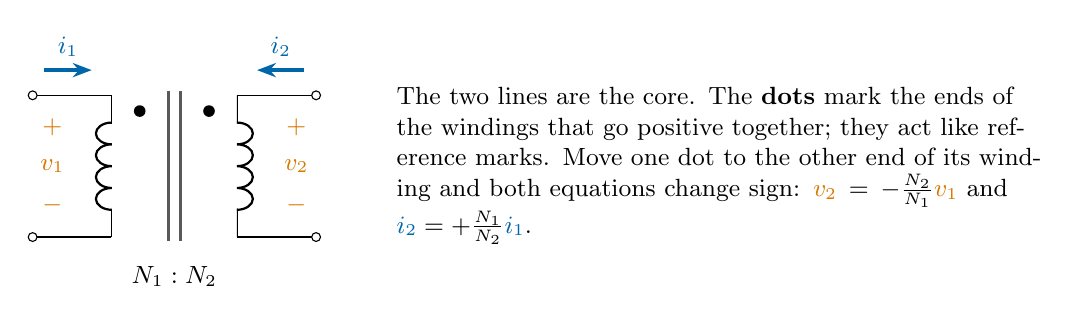
\begin{tikzpicture}[scale=1.0]
  \xfmr{0}{1.8}
  \draw (0,1.8) -- (-1.0,1.8) node[ocirc]{};  \draw (0,0) -- (-1.0,0) node[ocirc]{};
  \draw (1.6,1.8) -- (2.6,1.8) node[ocirc]{}; \draw (1.6,0) -- (2.6,0) node[ocirc]{};
  \node[pol] at (-0.75,1.4) {$+$}; \node[pol] at (-0.75,0.4) {$-$};
  \node[pol] at (-0.75,0.9) {$v_1$};
  \node[pol] at (2.35,1.4) {$+$}; \node[pol] at (2.35,0.4) {$-$};
  \node[pol] at (2.35,0.9) {$v_2$};
  \draw[iar] (-0.85,2.12) -- (-0.25,2.12); \node[font=\small, text=ccur] at (-0.55,2.42) {$i_1$};
  \draw[iar] (2.45,2.12) -- (1.85,2.12); \node[font=\small, text=ccur] at (2.15,2.42) {$i_2$};
  \node[font=\small] at (0.8,-0.5) {$N_1 : N_2$};
  \node[font=\small, anchor=west, text width=8.2cm] at (3.5,0.9)
    {The two lines are the core. The \textbf{dots} mark the ends of the windings that go
     positive together; they act like reference marks. Move one dot to the other end of
     its winding and both equations change sign:
     $\Vcol{v_2} = -\tfrac{N_2}{N_1}\Vcol{v_1}$ and
     $\Icol{i_2} = +\tfrac{N_1}{N_2}\Icol{i_1}$.};
\end{tikzpicture}
\end{center}

\subsection{Where the two equations come from}

\textbf{Voltages.} One flux $\Fcol{\Phi}$ passes through every turn of both windings. Each
turn therefore has the same voltage, $d\Fcol{\Phi}/dt$, and $N$ turns in series add up to
$\Vcol{v} = N\,d\Fcol{\Phi}/dt$. Divide by $N$:
\[
  \frac{\Vcol{v_1}}{N_1} \;=\; \frac{\Vcol{v_2}}{N_2} \;=\; \frac{d\Fcol{\Phi}}{dt} .
\]
\textbf{Currents.} An \emph{ideal} core needs no current at all to carry its flux. So the
windings' currents, each weighted by its number of turns, must cancel:
$N_1\Icol{i_1} + N_2\Icol{i_2} = 0$. A real core needs a small magnetising current; the
ideal one needs none.

\subsection{Any number of windings}

One core may carry $k$ windings. The same two arguments give one ratio for all of them and
one sum.

\begin{definitionbox}{Ideal transformer ($k$ windings)}
\[
  \frac{\Vcol{v_1}}{N_1} = \frac{\Vcol{v_2}}{N_2} = \cdots = \frac{\Vcol{v_k}}{N_k}
  \qquad\text{and}\qquad
  N_1\Icol{i_1} + N_2\Icol{i_2} + \cdots + N_k\Icol{i_k} = 0 ,
\]
every $\Vcol{v_j}$ positive and every $\Icol{i_j}$ entering at the dotted terminal of
winding~$j$.
\end{definitionbox}

\begin{cautionbox}[No derivatives --- and no DC]
The ideal transformer's equations are algebraic: no $d/dt$, no memory. It is a
\emph{resistive} element, listed with resistors and dependent sources in the course outline,
even though it is built from coils.\\[3pt]
A real transformer is not like that. It works only while the flux is changing. Feed it DC
and, once the current has settled, the flux is constant: the secondary voltage is zero and
the primary is just a coil --- a short circuit at DC, as in Lecture~5. Use the ideal model
for changing waveforms only.
\end{cautionbox}

%==============================================================
\section{The power of an ideal transformer}

Each winding has its reference arrow entering its $+$ terminal, so each obeys the PSC and
$\Vcol{v_j}\Icol{i_j}$ is the power that winding absorbs.

\begin{definitionbox}{The ideal transformer absorbs no power}
At every instant,
\[
  \Pcol{p(t)} \;=\; \sum_{j=1}^{k} \Vcol{v_j}\Icol{i_j} \;=\; 0 .
\]
\end{definitionbox}

\textbf{Proof.} Call the common ratio $\lambda(t) = \Vcol{v_j}/N_j$, the same for every $j$.
Then $\Vcol{v_j} = N_j\lambda$, and
\[
  \sum_{j=1}^{k} \Vcol{v_j}\Icol{i_j}
  \;=\; \sum_{j=1}^{k} N_j\lambda\,\Icol{i_j}
  \;=\; \lambda \sum_{j=1}^{k} N_j\Icol{i_j}
  \;=\; \lambda \cdot 0 \;=\; 0 . \qquad\blacksquare
\]
The first equation gave the common $\lambda$; the second made the sum vanish. Both are
needed.

\begin{center}
\small
\begin{tabular}{@{}l l l@{}}
\toprule
\textbf{Element} & \textbf{Absorbed power} & \textbf{What happens to the energy}\\
\midrule
resistor          & $\Pcol{p} \ge 0$          & dissipated\\
capacitor, inductor & $\Pcol{p}$ can change sign & stored, then returned\\
ideal transformer & $\Pcol{p} = 0$ at every instant & passed straight through\\
\bottomrule
\end{tabular}
\end{center}

With two windings, $\Vcol{v_1}\Icol{i_1} = -\Vcol{v_2}\Icol{i_2}$: whatever enters the
primary leaves the secondary at the same instant. The voltage is multiplied by $N_2/N_1$
and the current divided by the same factor, so the product is unchanged.

\begin{examplebox}[Example 6.4 --- a step-down transformer]
A $10:1$ transformer connects $v_s(t) = 120\cos\omega t\V$ to a $3\ohm$ load. Find the
currents and the power on each side.

\begin{center}
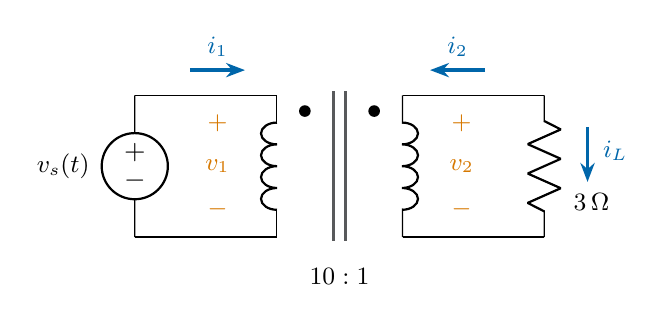
\begin{tikzpicture}[scale=1.0]
  \draw (-1.8,0) to[american voltage source, invert] (-1.8,1.8);
  \node[font=\small, left] at (-2.25,0.9) {$v_s(t)$};
  \draw (-1.8,1.8) -- (0,1.8); \draw (-1.8,0) -- (0,0);
  \xfmr{0}{1.8}
  \draw (1.6,1.8) -- (3.4,1.8); \draw (1.6,0) -- (3.4,0);
  \draw (3.4,1.8) to[R] (3.4,0);
  \node[font=\small, right] at (3.65,0.45) {$3\ohm$};
  \draw[iar] (3.95,1.4) -- (3.95,0.7); \node[font=\small, text=ccur] at (4.3,1.1) {$i_L$};
  \node[pol] at (-0.75,1.45) {$+$}; \node[pol] at (-0.75,0.9) {$v_1$}; \node[pol] at (-0.75,0.35) {$-$};
  \node[pol] at (2.35,1.45) {$+$}; \node[pol] at (2.35,0.9) {$v_2$}; \node[pol] at (2.35,0.35) {$-$};
  \draw[iar] (-1.1,2.12) -- (-0.4,2.12); \node[font=\small, text=ccur] at (-0.75,2.42) {$i_1$};
  \draw[iar] (2.65,2.12) -- (1.95,2.12); \node[font=\small, text=ccur] at (2.3,2.42) {$i_2$};
  \node[font=\small] at (0.8,-0.5) {$10 : 1$};
\end{tikzpicture}
\end{center}

\textbf{Voltages.} $\Vcol{v_1} = 120\cos\omega t\V$, so
$\Vcol{v_2} = \tfrac{1}{10}\Vcol{v_1} = 12\cos\omega t\V$.

\textbf{Currents.} The load takes $\Icol{i_L} = \Vcol{v_2}/3 = 4\cos\omega t\A$. That current
leaves the dotted terminal, so $\Icol{i_2} = -4\cos\omega t\A$, and
$\Icol{i_1} = -\tfrac{N_2}{N_1}\Icol{i_2} = 0.4\cos\omega t\A$.

\textbf{Power.}
\[
  \Pcol{p_1} = \Vcol{v_1}\Icol{i_1} = 48\cos^2\omega t\W ,
  \qquad
  \Pcol{p_2} = \Vcol{v_2}\Icol{i_2} = -48\cos^2\omega t\W ,
  \qquad
  \Pcol{p_1} + \Pcol{p_2} = 0 .
\]
The primary takes $48\cos^2\omega t\W$ from the source and the secondary hands exactly that
to the load --- at every instant, not only on average.

\textbf{Seen from the source.} $\Vcol{v_1}/\Icol{i_1} = 120/0.4 = 300\ohm$. The source cannot
tell the transformer and the $3\ohm$ load from a single $300\ohm$ resistor, and
$300 = 10^2 \times 3$.
\end{examplebox}

The last line is general. With $\Vcol{v_1} = \tfrac{N_1}{N_2}\Vcol{v_2}$,
$\Icol{i_1} = \tfrac{N_2}{N_1}\Icol{i_L}$ and $\Vcol{v_2} = R_L\Icol{i_L}$,
\[
  \frac{\Vcol{v_1}}{\Icol{i_1}} \;=\; \Bigl(\frac{N_1}{N_2}\Bigr)^{\!2} R_L .
\]
A transformer \emph{rescales resistance} by the square of its turns ratio. That is how an
$8\ohm$ loudspeaker is made to look like a much larger resistance to the amplifier that
drives it.

%==============================================================
\section{A transformer is two dependent sources}

The two equations of the ideal transformer can be read as two dependent sources. The
secondary is a VCVS controlled by $\Vcol{v_1}$; the primary is a CCCS controlled by
$\Icol{i_2}$.

\begin{center}
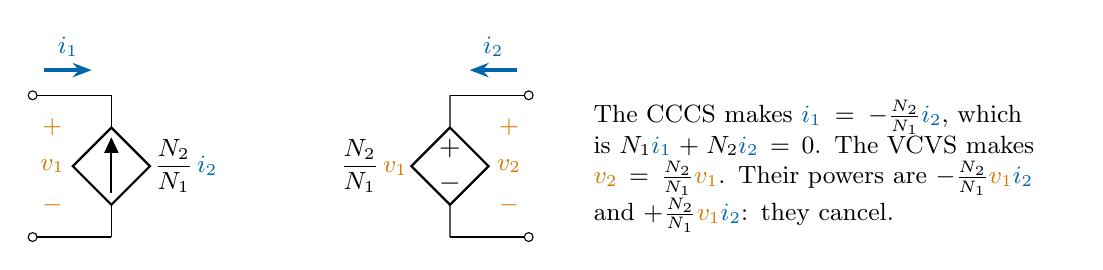
\begin{tikzpicture}[scale=1.0]
  \draw (0,0) to[american controlled current source] (0,1.8);
  \node[font=\small, right] at (0.42,0.9) {$\dfrac{N_2}{N_1}\,\Icol{i_2}$};
  \draw (0,1.8) -- (-1.0,1.8) node[ocirc]{}; \draw (0,0) -- (-1.0,0) node[ocirc]{};
  \node[pol] at (-0.75,1.4) {$+$}; \node[pol] at (-0.75,0.4) {$-$};
  \node[pol] at (-0.75,0.9) {$v_1$};
  \draw[iar] (-0.85,2.12) -- (-0.25,2.12); \node[font=\small, text=ccur] at (-0.55,2.42) {$i_1$};
  \draw (4.3,0) to[american controlled voltage source, invert] (4.3,1.8);
  \node[font=\small, left] at (3.88,0.9) {$\dfrac{N_2}{N_1}\,\Vcol{v_1}$};
  \draw (4.3,1.8) -- (5.3,1.8) node[ocirc]{}; \draw (4.3,0) -- (5.3,0) node[ocirc]{};
  \node[pol] at (5.05,1.4) {$+$}; \node[pol] at (5.05,0.4) {$-$};
  \node[pol] at (5.05,0.9) {$v_2$};
  \draw[iar] (5.15,2.12) -- (4.55,2.12); \node[font=\small, text=ccur] at (4.85,2.42) {$i_2$};
  \node[font=\small, anchor=west, text width=6.0cm] at (6.0,0.9)
    {The CCCS makes $\Icol{i_1} = -\tfrac{N_2}{N_1}\Icol{i_2}$, which is
     $N_1\Icol{i_1} + N_2\Icol{i_2} = 0$. The VCVS makes
     $\Vcol{v_2} = \tfrac{N_2}{N_1}\Vcol{v_1}$. Their powers are
     $-\tfrac{N_2}{N_1}\Vcol{v_1}\Icol{i_2}$ and $+\tfrac{N_2}{N_1}\Vcol{v_1}\Icol{i_2}$:
     they cancel.};
\end{tikzpicture}
\end{center}

This links the two halves of the lecture. Each dependent source on its own can deliver
power; in this pair one always delivers exactly what the other absorbs.

%==============================================================
\section*{Summary}
\addcontentsline{toc}{section}{Summary}

\begin{center}
\small
\begin{tabular}{@{}l l l@{}}
\toprule
\textbf{Element} & \textbf{Terminal equations} & \textbf{Power}\\
\midrule
VCVS, CCVS & $\Vcol{v} = \mu\Vcol{v_1}$, \ $\Vcol{v} = r\Icol{i_1}$ & can deliver (active)\\
VCCS, CCCS & $\Icol{i} = g\Vcol{v_1}$, \ $\Icol{i} = \beta\Icol{i_1}$ & can deliver (active)\\
ideal transformer & $\Vcol{v_j}/N_j$ all equal, \ $\sum_j N_j\Icol{i_j} = 0$ & $\Pcol{p} = 0$ at every instant\\
\bottomrule
\end{tabular}
\end{center}

\begin{itemize}
  \item A \textbf{dependent source} (diamond) takes its value from a voltage or current in
        another branch. Four kinds: VCVS, CCVS, VCCS, CCCS; the constant's unit is output
        over input.
  \item Its terminal equation names a \textbf{foreign variable}. Otherwise nothing
        changes: write KCL, KVL and terminal equations, plus one equation for the
        controlling variable.
  \item It can \textbf{deliver power} --- that is what amplification is --- but it
        \textbf{cannot start anything}: without an independent source everything is zero.
        It is never switched off.
  \item The \textbf{ideal transformer}: $\Vcol{v_1}/N_1 = \Vcol{v_2}/N_2$ and
        $N_1\Icol{i_1} + N_2\Icol{i_2} = 0$, with signs set by the \textbf{dots}. It is
        resistive (no $d/dt$), but a real one needs changing waveforms.
  \item It \textbf{absorbs no power at any instant}, and it rescales a load resistance by
        $(N_1/N_2)^2$.
\end{itemize}

\subsection*{Next lecture}
From circuit to \textbf{graph}: labelling the nodes and branches of a circuit so that its
$2b$ equations can be written systematically --- the first step towards node and mesh
analysis.

\subsection*{Reading}
\begin{itemize}
  \item Alexander \& Sadiku, \emph{Fundamentals of Electric Circuits}, Section~1.6
        (dependent sources) and Section~13.5 (ideal transformers).
  \item Chua, Desoer \& Kuh, \emph{Linear and Nonlinear Circuits} --- controlled sources
        and the ideal transformer.
  \item Lecture notes and videos of Prof.\ Emre Tuna,
        \href{https://users.metu.edu.tr/etuna/ee201/}{\texttt{users.metu.edu.tr/etuna/ee201}}
        --- notes p.~11; Lecture~5 video: dependent sources $41{:}47$, the four kinds
        $43{:}04$--$48{:}14$, example $49{:}15$, ideal transformer $51{:}31$, its power
        $54{:}47$.
\end{itemize}

\end{document}
